\section{Ejercicio 2}

Para familiarizarnos con el formato de lote de tareas y el funcionamiento del simulador, ejecutamos el conjunto de tareas presentado en el Lote \ref{fig:lote-ejercicio-2} utilizando el scheduler de tipo \textbf{FCFS}. El lote presenta una tarea tipo \textit{TaskCPU}, que hace uso del CPU exclusivamente, y dos tareas tipo \textit{TaskConsola}, que adicionalmente realizan llamados bloqueantes de entrada/salida.

\begin{minipage}[t]{0.5\textwidth}
  \begin{tarea}[H]
    \vspace*{2mm}
    \begin{verbatim}
    @0:
    TaskCPU 25
    TaskConsola 5 1 11
    TaskConsola 10 2 3
    \end{verbatim}
    \vspace*{-5mm}
  \caption{Lote de tareas para evaluar el scheduler \textbf{FCFS} con 1, 2 y 3 núcleos.}
  \label{fig:lote-ejercicio-2}
  \end{tarea}
\end{minipage}\\\\

El lote se simuló utilizando 1, 2 y 3 núcleos, manteniendo fijo el costo de cambio de contexto y migración de procesos en 1 tick cada uno; en las figuras \ref{fig:ejercicio-2-1-nucleos}, \ref{fig:ejercicio-2-2-nucleos} y \ref{fig:ejercicio-2-3-nucleos} se observan los diagramas de Gantt correspondientes a cada simulación.

\begin{figure}[h!t]
  \centering
  \makebox[\textwidth][c]{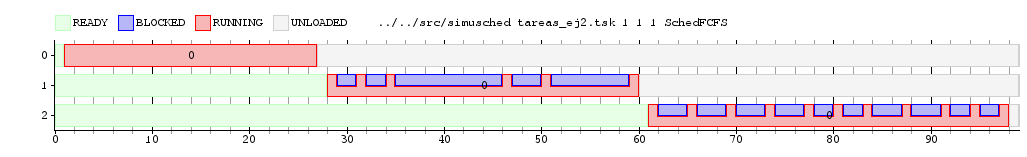
\includegraphics[width=1.2\textwidth]{graphics/tareas_ej2_1_1_1_fcfs.png}}%
  \caption{Ejecución del Lote \ref{fig:lote-ejercicio-2} ejecutándose en \textbf{FCFS} con 1 núcleo.}
  \label{fig:ejercicio-2-1-nucleos}
\end{figure}

\begin{figure}[h!t]
  \centering
  \makebox[\textwidth][c]{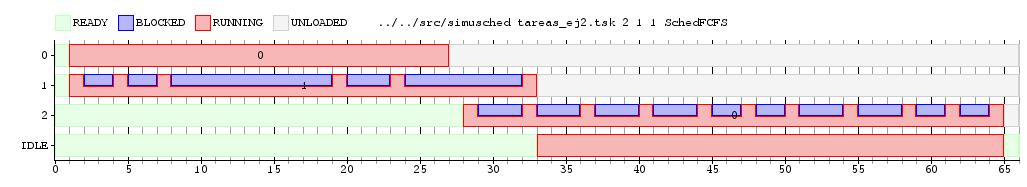
\includegraphics[width=1.2\textwidth]{graphics/tareas_ej2_2_1_1_fcfs.png}}%
  \caption{Ejecución del Lote \ref{fig:lote-ejercicio-2} ejecutándose en \textbf{FCFS} con 2 núcleos.}
  \label{fig:ejercicio-2-2-nucleos}
\end{figure}

\begin{figure}[h!t]
  \centering
  \makebox[\textwidth][c]{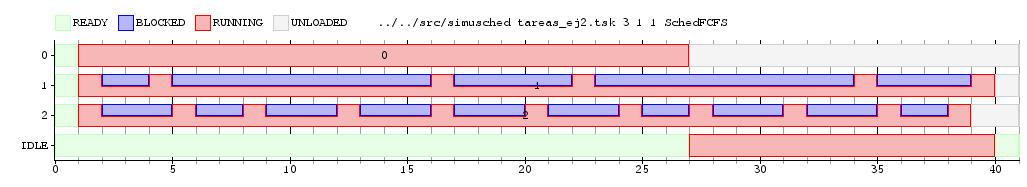
\includegraphics[width=1.2\textwidth]{graphics/tareas_ej2_3_1_1_fcfs.png}}%
  \caption{Ejecución del Lote \ref{fig:lote-ejercicio-2} ejecutándose en \textbf{FCFS} con 3 núcleos.}
  \label{fig:ejercicio-2-3-nucleos}
\end{figure}

En los diagramas presentados se observa que el scheduler tipo \textbf{FCFS} efectivamente asigna las tareas en el orden que se declaran en el lote. Las tareas tienen posesión sobre el núcleo donde son asignadas desde el comienzo hasta el final de su ejecución, independientemente de los llamados bloqueantes de entrada/salida que realicen, o las tareas aguardando en estado \textit{ready}.